
\chapter{Results}
\label{ch:results}

% Present the results of data generation experiments, including visual inspection, statistical analysis, and correlation with real data.
\section{First Dataset}


\subsection{Statistical Distribution}



The patient's age and disease will be studied, as the difference between the models is clearly illustrated.

\begin{figure}[H]
    \centering
    \begin{subfigure}[b]{0.45\textwidth}
        \centering
        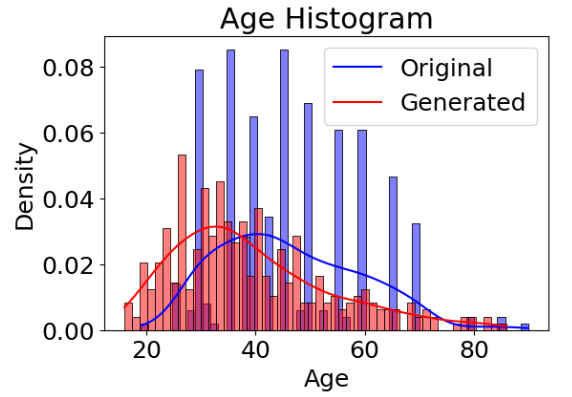
\includegraphics[width=\textwidth]{images/age_ctgan.png}
        \caption{CTGAN}
        \label{fig:age_ctgan}
    \end{subfigure}
    \hfill
    \begin{subfigure}[b]{0.45\textwidth}
        \centering
        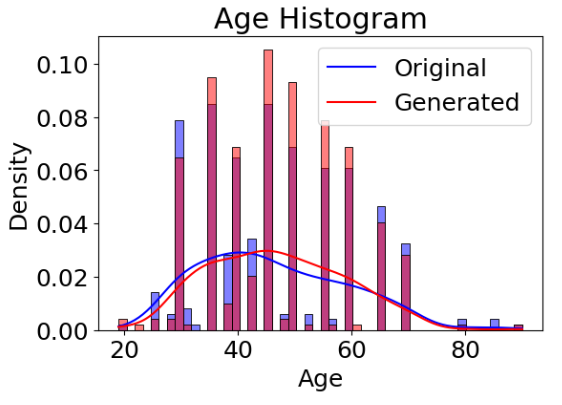
\includegraphics[width=\textwidth]{images/age_begreat.png}
        \caption{BeGreat}
        \label{fig:age_begreat}
    \end{subfigure}
    \hfill
    \begin{subfigure}[b]{0.45\textwidth}
        \centering
        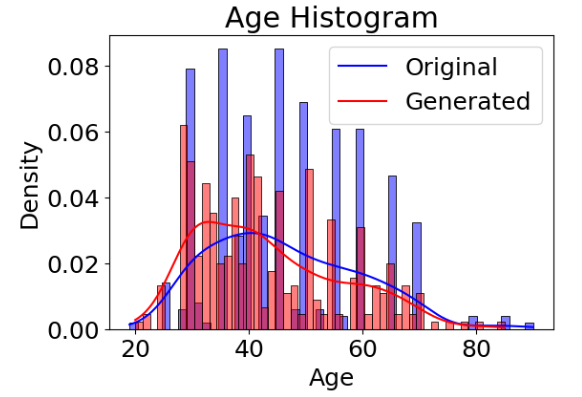
\includegraphics[width=\textwidth]{images/age_llama.png}
        \caption{LLaMa-3}
        \label{fig:age_llama}
    \end{subfigure}
    \caption{Age Distribution for Different Models}
    \label{fig:age_distrib}
\end{figure}

From figure \ref{fig:age_distrib}, the density curve \ref{fig:age_ctgan} shows that the CTGAN model can capture the dominant patient age demographic. Nonetheless, there is a slight variation compared to the original data.
The density curves, from \ref{fig:age_begreat}, indicate an almost perfect alignment between the generated data and the original data, showcasing the model's effectiveness in replicating the age distribution. The density curve from the LLaMa-3 model (\ref{fig:age_llama}) shows a very close alignment with the original data, but it is still better compared to the CTGAN and not as precise as the BeGreat model.


\begin{figure}[H]
    \centering
    \begin{subfigure}[b]{0.45\textwidth}
        \centering
        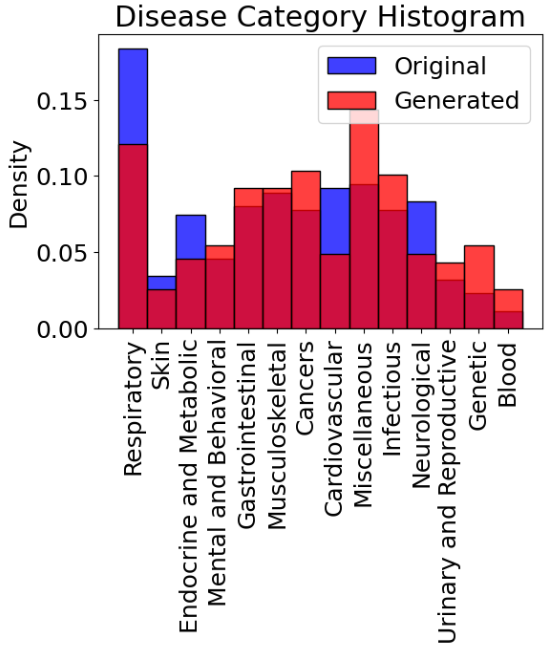
\includegraphics[width=\textwidth]{images/disease_ctgan.png}
        \caption{CTGAN}
        \label{fig:disease_ctgan}
    \end{subfigure}
    \hfill
    \begin{subfigure}[b]{0.45\textwidth}
        \centering
        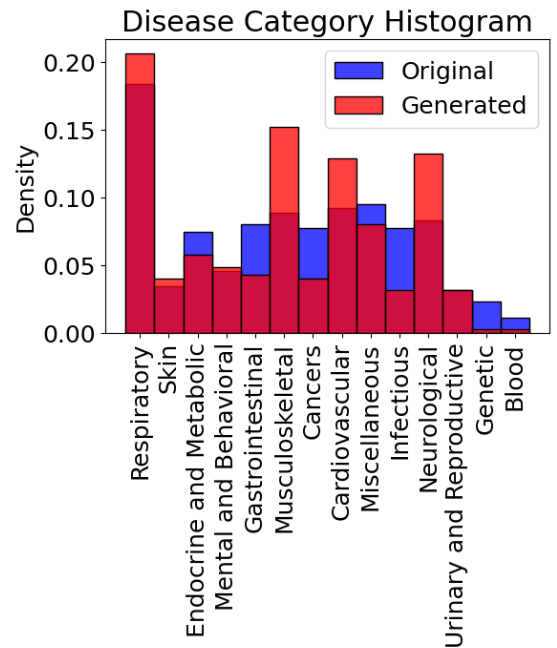
\includegraphics[width=\textwidth]{images/disease_begreat.png}
        \caption{BeGreat}
        \label{fig:disease_begreat}
    \end{subfigure}
    \hfill
    \begin{subfigure}[b]{0.45\textwidth}
        \centering
        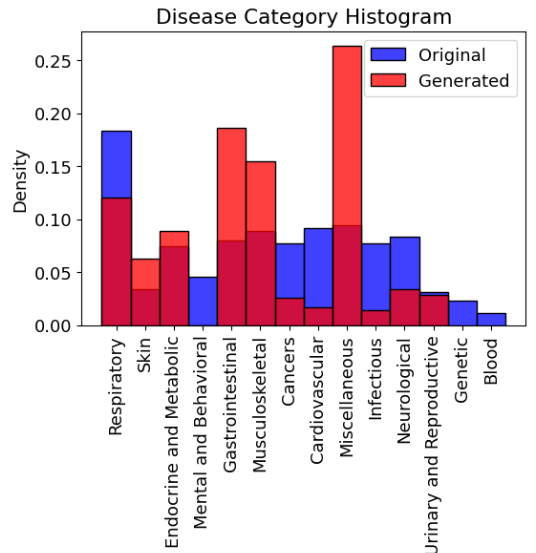
\includegraphics[width=\textwidth]{images/disease_llama.png}
        \caption{LLaMa-3}
        \label{fig:disease_llama}
    \end{subfigure}
    \caption{Comparison of Disease Categories Between Original and Generated Data for Different Models}
    \label{fig:disease_distrib}
\end{figure}

Figure \ref{fig:disease_distrib} illustrates the disease distribution from the original and synthetic data. CTGAN (\ref{fig:disease_ctgan}) as well as BeGreat (\ref{fig:disease_begreat}) replicate almost identical to the original data. However, LLaMa-3 (\ref{fig:disease_llama}) suggests a more different and diverse range of diseases with a high density for the miscellaneous category. LLaMa-3 was given a prompt where was asked the model to generate new diseases, which is why there is a higher density in the miscellaneous category.

\vspace{1cm}

\noindent \textsc{ \textbf{Summary}}

The analysis of the statistical distribution of the synthetic data reveals that the BeGreat model provides the generated data that is closest to the original data by replicating the distribution of the variables. The CTGAN model struggles to capture the distribution of the original data as it shows slight variations in figure \ref{fig:age_distrib}, but was able to replicate the disease category distribution. Finally, despite the LLaMa-3 model showing good match in the age distribution, due to the prompt given to the model, it had generated a diverse range of new diseases categorized as 'miscellaneous' which is why the generated data is statistically different from the real data.
These findings highlight that LLM models is the most effective in replicating the real data's distribution compared to the GAN-based models.


\subsection{Comparative Analysis of Original and Synthetic Data}


\begin{figure}[H]
    \centering
    \begin{subfigure}[b]{0.45\textwidth}
        \centering
        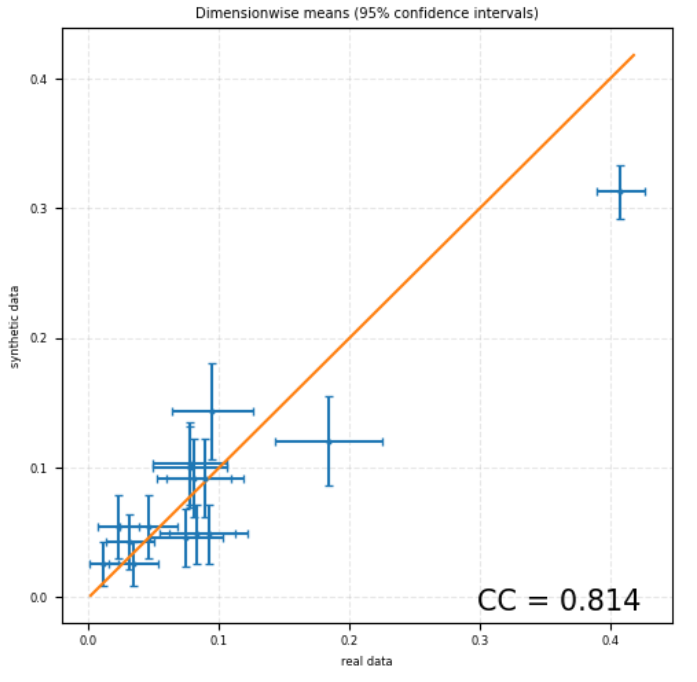
\includegraphics[width=\textwidth]{images/avg_dim_ctgan.png}
        \caption{CTGAN}
        \label{fig:avg_dim_ctgan}
    \end{subfigure}
    \hfill
    \begin{subfigure}[b]{0.45\textwidth}
        \centering
        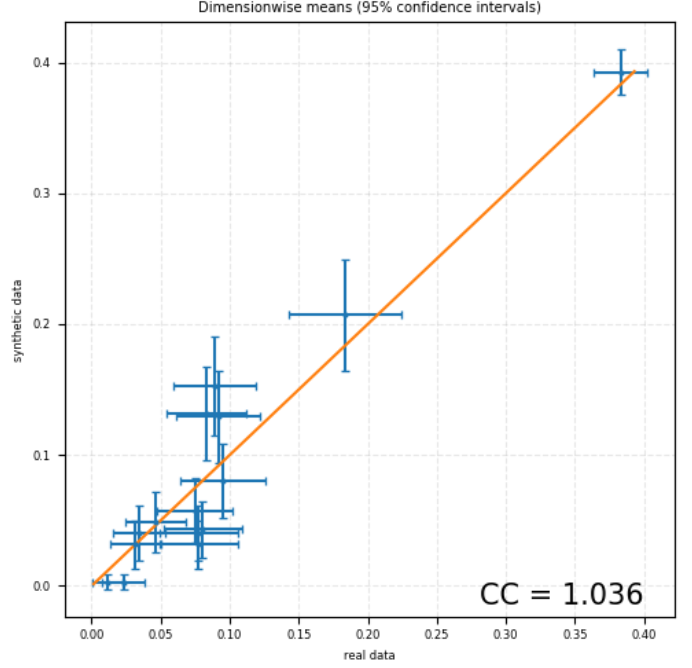
\includegraphics[width=\textwidth]{images/avg_dim_begreat.png}
        \caption{BeGreat}
        \label{fig:avg_dim_begreat}
    \end{subfigure}
    \hfill
    \begin{subfigure}[b]{0.48\textwidth}
        \centering
        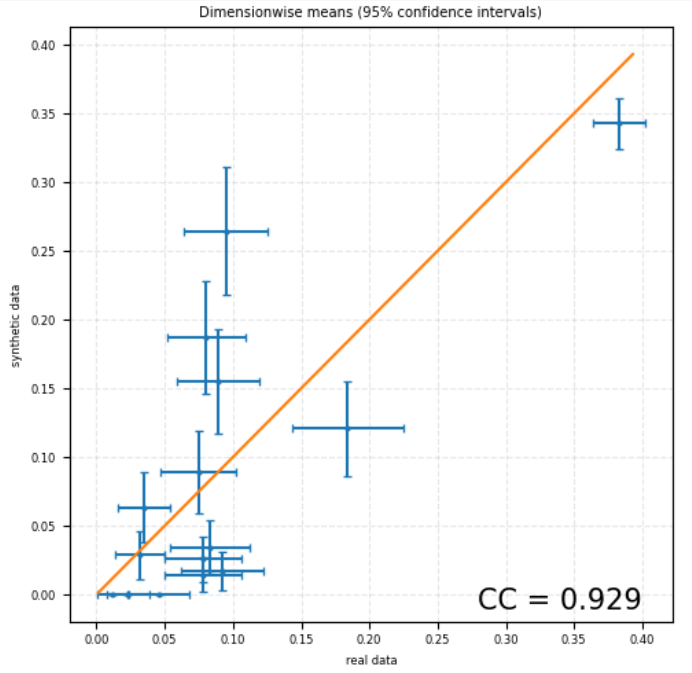
\includegraphics[width=\textwidth]{images/avg_dim_llama.png}
        \caption{LLaMa-3}
        \label{fig:avg_dim_llama}
    \end{subfigure}
    \caption{Dimensionwise means (95\% confidence intervals) scatter plots for different models}
    \label{fig:dim_means_distrib}
\end{figure}

Figure \ref{fig:dim_means_distrib} shows different scatter plots of the dimensionwise means with 95\% confidence intervals. The CTGAN model (\ref{fig:avg_dim_ctgan}) shows a correlation coefficient of 0.814, demonstrating that the model can synthesize correlated data to the original data with a high concentration of points in the lower values. However, the BeGreat model (\ref{fig:avg_dim_begreat}) has a correlation value of 1.036 which shows a perfect correlation between the synthetic and original data. This strong correlation can also be seen in the distribution \ref{fig:age_begreat}. LLaMa-3 has a correlation coefficient of 0.929 (\ref{fig:avg_dim_llama}), indicating that the model could capture the complex distribution of the original data. 



\vspace{0.5cm}


\begin{figure}[H]
    \centering
        \centering
        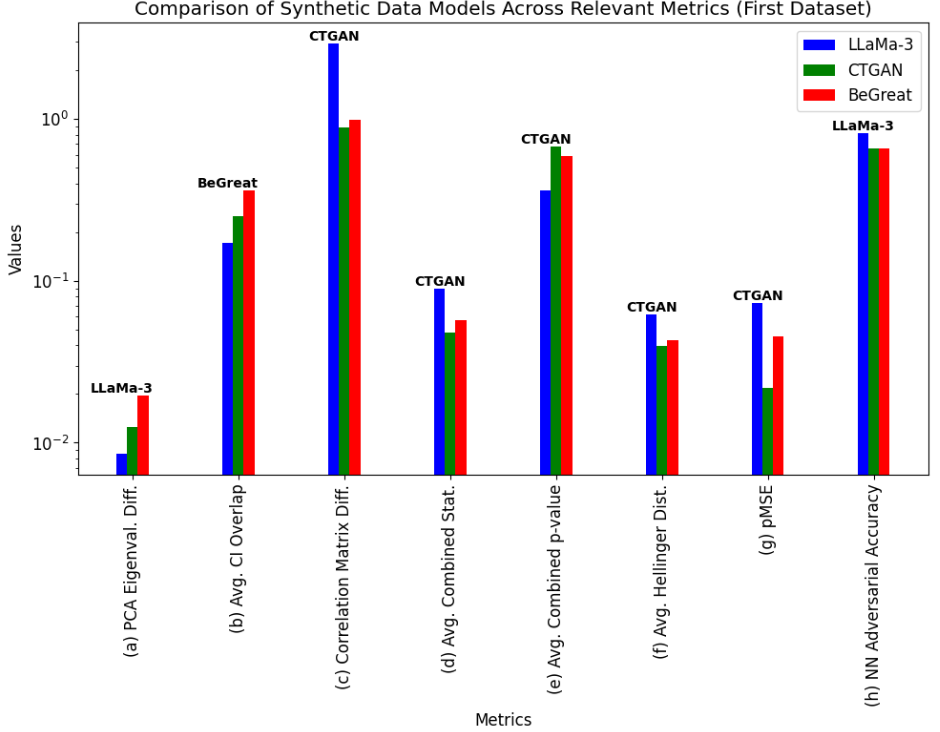
\includegraphics[width=1\textwidth]{images/dataset1_metrics.png}
        \caption{Comparison of synthetic data models across different metrics for the first dataset. In blue, LLaMa-3, in green CTGAN, in red BeGreat.}
        \label{fig:dataset1_metrics}
\end{figure}

\begin{enumerate}
    \item[(a)] PCA Eigenvalue Difference \\
    LLaMa-3 has the lowest PCA Eigenvalue Difference suggesting it best captures the variance of the original data. 

    \item[(b)] Average Confidence Interval Overlap \\
    BeGreat shows the highest average CI overlap indicating its consistency in preserving variability of the original data.

    \item[(c)] Correlation Matrix Difference \\
    CTGAN model preserves better the relationships between variables.

    \item[(d \& e)] Average Combined Statistics \& Average Combined p-value \\
    CTGAN model has the lowest value for the average combined statistics and the highest average combined p-value which both indicate the closest distributional match.

    \item[(f)] Average Hellinger Distance \\
    CTGAN model shows the lowest average Hellinger distance value indicating the closest match to the original data’s distribution.

    \item[(g)] pMSE \\
    CTGAN has low pMSE values, indicating it effectively replicates the original data. 

    \item[(h)] NN Adversarial Accuracy \\
    Llama3 shows high adversarial accuracy, indicating variability in distinguishability.
\end{enumerate}

More detailed results can be found in the following appendix \ref{}

\vspace{1cm}

\noindent \textsc{ \textbf{Summary}}

The comparison of the synthetic data models across the dimensionwise means shows that LLMs generated more correlated data compared to GAN-based models. In this case, the BeGreat model provided strong performance in replicating dimensionwise means of the original data. As for the other metrics, LLMs were able to capture the variance of the real data and preserve the variability between variables. The LLaMa-3, due to its distinct values of the generated data gave a strong variability in distinguishability. However, LLMs performed less well in other specificity of the real data where GAN-based models excelled. The CTGAN model showed the closest distributional match to the original data.


\subsection{Classification Accuracy Test Results}

The generated data consists of only 348 individual records, which is considered very low for training and evaluating machine learning models. A small training sample can lead to inaccuracies and biased outcomes. 


\begin{figure}[H]
    \centering
        \centering
        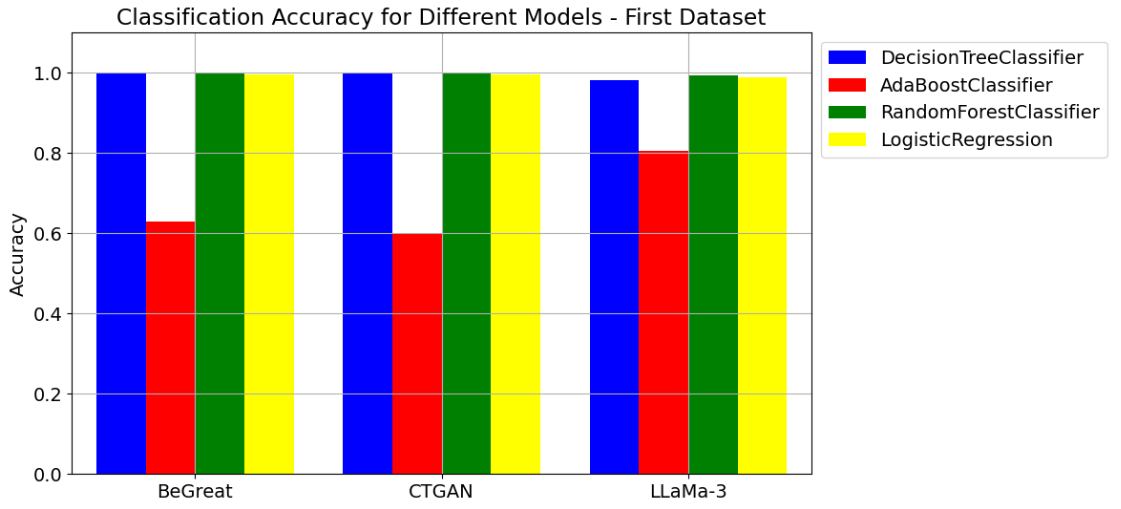
\includegraphics[width=1\textwidth]{images/dataset1_ml.png}
        \caption{Comparison of classification accuracy across machine learning models for the first dataset using Decision Tree Classifier, AdaBoost Classifier, Random Forest Classifier, and Logistic Regression.}
        \label{fig:dataset1_ml}
\end{figure}

Figure \ref{fig:dataset1_ml} shows the performance of different machine learning models using the first dataset. The decision tree, random forest classifiers and the logistic regression all show high accuracies. This is highly due to the fact that the model has been trained on a small sample and cannot give consistent and accurate results. However, the AdaBoost classifier was able to capture the difference lying in the different generated data. LLaMa-3 is outperforming both BeGreat and CTGAN and demonstrates the highest overall accuracies. The same goes for the BeGreat model it was able to perform better than CTGAN.



\subsection{Privacy Metrics Comparison}

For better visualization, the results of the data privacy metrics are normalized. 


\begin{figure}[H]
    \centering
        \centering
        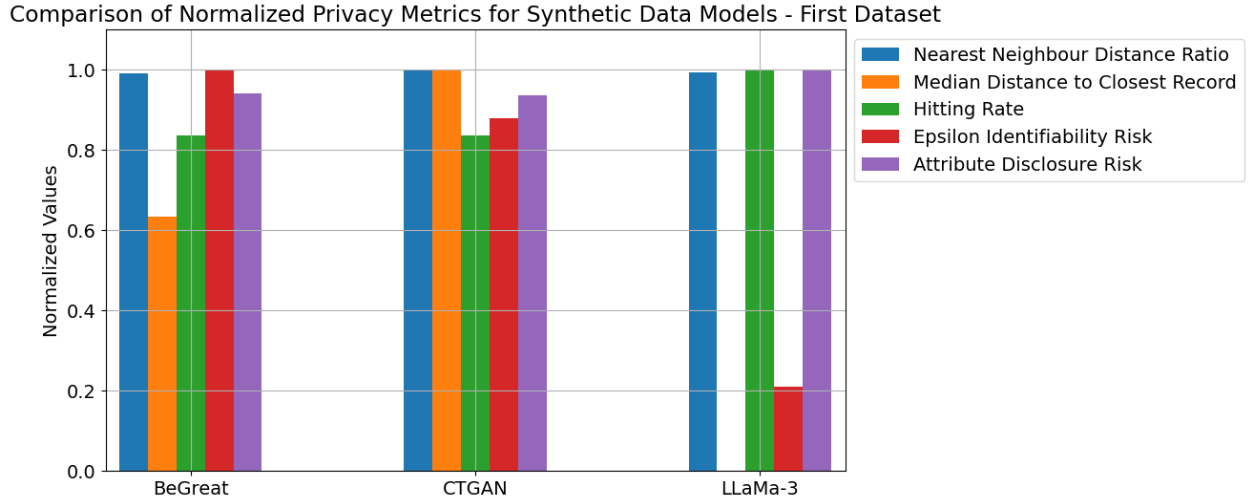
\includegraphics[width=1\textwidth]{images/dataset1_privacy.png}
        \caption{Comparison of normalised privacy metrics for synthetic data models in the first dataset.}
        \label{fig:dataset1_privacy}
\end{figure}

Figure \ref{fig:dataset1_privacy} shows various privacy metrics results of the different models.

\begin{enumerate}
    \item[(a)] Nearest Neighbour Distance Ratio \\
    All models show very close values to 1.0. However, a high value of the neatest neighbour distance ratio indicates a low privacy. Digging into the precise values of the metric, which can be found in the appendix, the BeGreat suggests a lower value compared to the other two models. Nonetheless, data privacy is not respected for all models for that particular metric.

    \item[(b)] Median Distance to Closest Record \\
    CTGAN shows the highest median distance to the closest record, indicating the best privacy. Model BeGreat follows after the CTGAN model, while Model Llama3 has an infinite median distance, suggesting perfect privacy. % need to be checked

    
    \item[(c)] Hitting Rate \\
    LLaMa-3 suggests a higher hitting rate (0.0172), indicating slightly low privacy. BeGreat and CTGAN show the lowest hitting rate (0.0144), indicating better privacy. However, all hitting rates are close to the value 0 which in that case the normalization is not suited for this metric. Thus, all models contribute to better data privacy.


    \item[(d)] Epsilon Identifiability Risk \\
    LLaMa-3 shows the lowest epsilon identifiability risk (0.0805), followed by CTGAN (0.3381). BeGreat has the highest risk (0.3849). CTGAN and BeGreat have almost the same risk value, which suggests lower privacy. On the other hand, LLaMa-3 has a value much closer to 0, indicating that it performs better at generating data with a low risk of exposing real information. 

    \item[(e)] Attribute Disclosure Risk \\
    CTGAN shows the lowest attribute disclosure risk (0.7993), followed closely by BeGreat (0.8044). Llama3 has the highest risk (0.8540), indicating lower privacy. However, all models have a relatively high value of the attribute disclosure risk, which suggests they are as vulnerable as the others. %% better reformulation
    
\end{enumerate}

\vspace{1cm}

\noindent \textsc{ \textbf{Summary}}

The privacy metrics comparison shows that both LLMs and GAN-based models have similar results in terms of privacy. Results indicate that all models tend to generate data that is close to the real data, which can lead to privacy concerns depicted in (a), (d) and (e). However, the LLaMa-3 model shows better privacy in terms of (b) and (d). The BeGreat model shows better privacy in terms of (a) and (e). The CTGAN model shows better privacy in terms of (c). The results suggest that the LLaMa-3 model is the most effective in preserving privacy, while the BeGreat model also performs well in certain metrics. The CTGAN model shows mixed results across different metrics, indicating variability in its effectiveness in preserving privacy.

\vspace{1cm}

\noindent \textsc{ \textbf{Conclusion for the first dataset}}

The utilization of the first dataset has shown that LLMs are more effective in replicating the real data's distribution, its correlation between variables and its complex structure as indicated by the different metrics and machine learning results. The GAN-based models, on the other hand, struggles to effectively capture the real data's distribution but was able to replicate the distribution with a some variations. Both models have shown mixed results in data privacy. Note that LLaMa-3 has generated distinct data which somewhat improved the data privacy.

%%%%%%%%%%%%%%%%%%%%%%%%%%%%%%%%%%%%%%%%%%%%%%%%%%%%%%%%%%%%%%%%%%%%%%%%%%%%%%%%%%%%%%%%%%%%%%%%%%%%%%%%%%%%%%%%%%%%%%%%%%%%%%%%%%%%%%%%%%%%%%%%%%%%%%%%%%%%%%%%%%%%%%%%%%%%%%%%%%%%%%%%%%%%%%%%%%%%%%%%%%%%%%%%%%%%%%%%%%%%%%%%%%%%%%%%%%%%%%%%%%%%%%%%%%%%%%%%%%%%%%%%%%%%%%%%%%%%%%%%%%%%%%%%%%%%%%%%%%%%%%%%%%%%%%%%%%%%%%%%%%%%%%%%%%%%%%%%%%%%%%%%%%%%%%%%%%%%%%%%%%%%%%%%%%%%%%%%%%%%%%%%%%%%%%%%%%%%%%%%%%%%%%%%%%%%%%%%%%%%%%%%%%%%%%%%%%%%%%%%%%%%%%%%%%%%%%%%%%%%



\section{Second Dataset}

\subsection{Statistical Distribution}

\subsection{Comparative Analysis of Original and Synthetic Data}

\begin{figure}[H]
    \centering
    \begin{subfigure}[b]{0.47\textwidth}
        \centering
        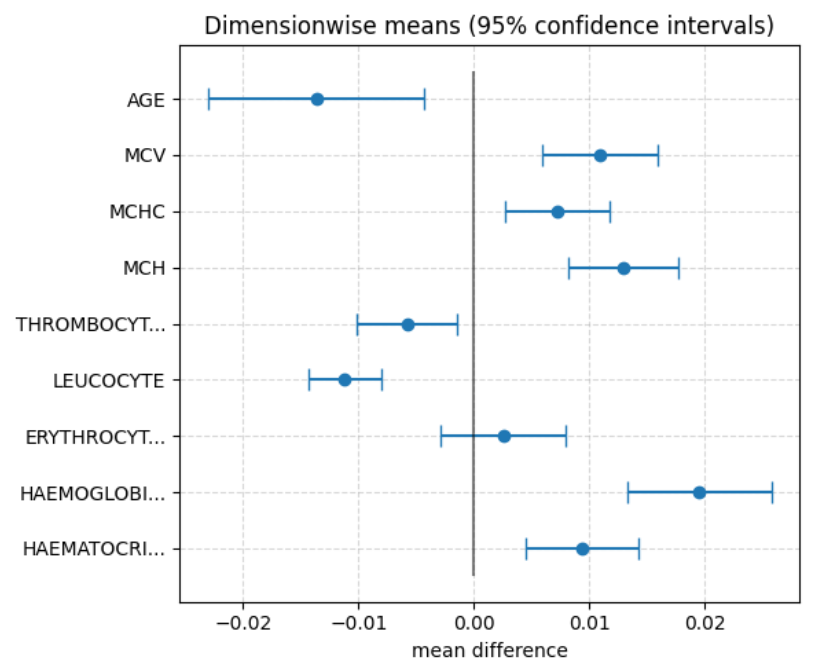
\includegraphics[width=\textwidth]{images/avg_dim_2_ctgan.png}
        \caption{CTGAN}
        \label{fig:avg_dim_2_ctgan}
    \end{subfigure}
    \hfill
    \begin{subfigure}[b]{0.47\textwidth}
        \centering
        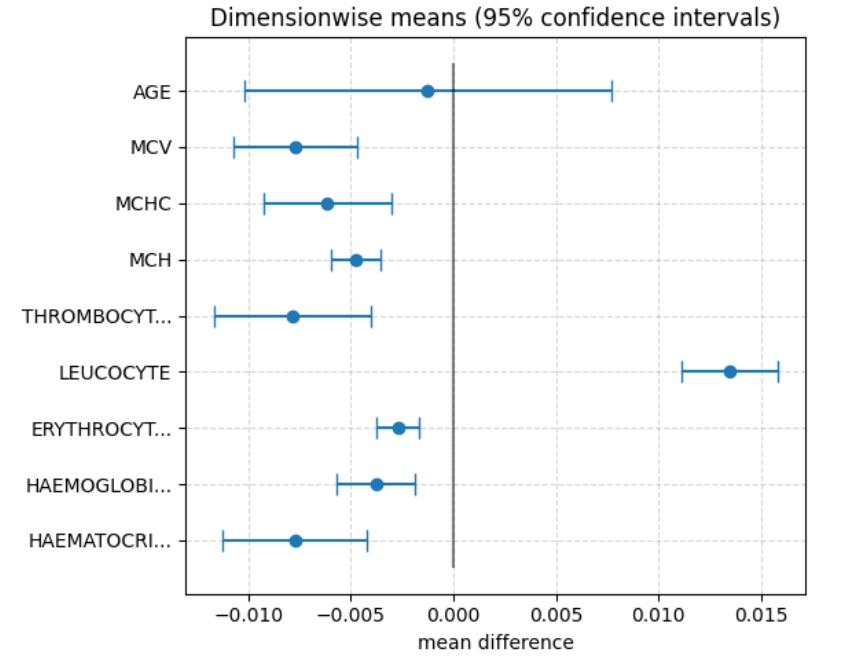
\includegraphics[width=\textwidth]{images/avg_dim_2_begreat.png}
        \caption{BeGreat}
        \label{fig:avg_dim_2_begreat}
    \end{subfigure}
    \hfill
    \begin{subfigure}[b]{0.48\textwidth}
        \centering
        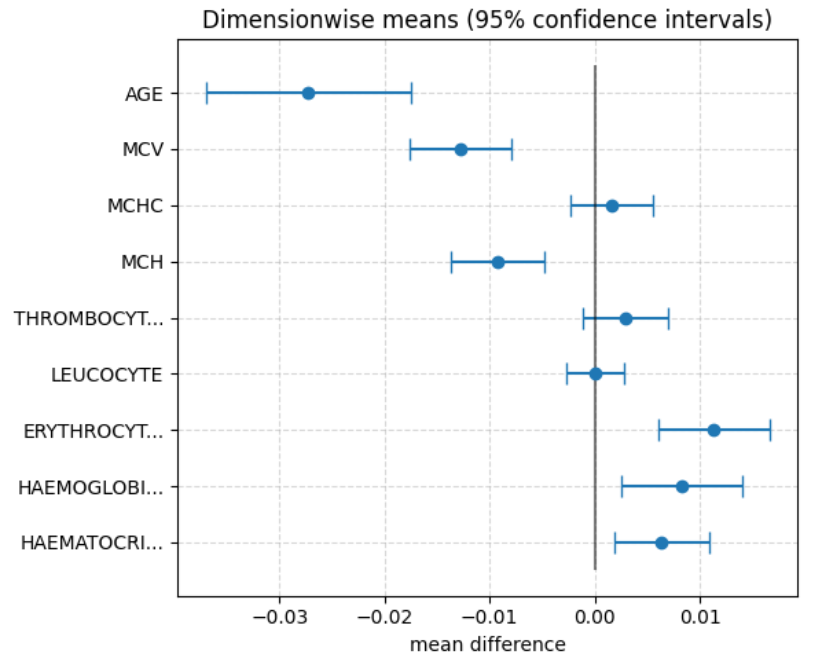
\includegraphics[width=\textwidth]{images/avg_dim_2_llama.png}
        \caption{LLaMa-3}
        \label{fig:avg_dim_2_llama}
    \end{subfigure}
    \caption{Dimensionwise means (95\% confidence intervals) mean-difference plot for different models}
    \label{fig:dim_means_distrib_2}
\end{figure}


Figure \ref{fig:dim_means_distrib_2} shows the mean-difference plots for different models. LLaMa-3 (\ref{fig:avg_dim_2_llama}) shows a drastic shift of the 'AGE' from the zero difference line (black vertical bar) showing that the model tends to generate more variability for the patient's age compared with the original data. On the other hand, the BeGreat model (\ref{fig:avg_dim_2_begreat}) shows a much closer 'AGE' variability from the original data. 
The BeGreat model shows relatively close values from the zero difference line for the other variables indicating that these variables are closer to the real data's variables. Conversely, the CTGAN and the LLaMa-3 model both depict more varied mean differences of variables such as MCV, ERYTHROCYTE etc... leading to more distinct data than the original data. 




\begin{figure}[H]
    \centering
        \centering
        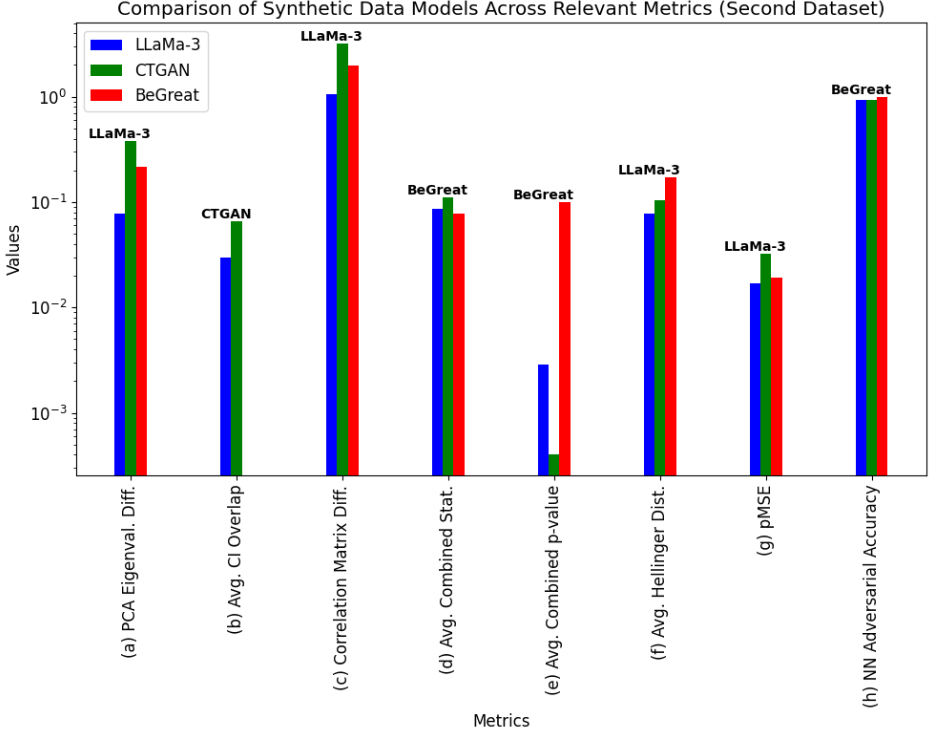
\includegraphics[width=1\textwidth]{images/dataset2_metrics.png}
        \caption{Comparison of synthetic data models across different metrics for the second dataset. In blue, LLaMa-3, in green CTGAN, in red BeGreat.}
        \label{fig:dataset2_metrics}
\end{figure}

\begin{enumerate}
    \item[(a)] PCA Eigenvalue Difference \\
    LLaMa-3 has the lowest PCA Eigenvalue Difference suggesting it best captures the variance of the original data. 

    \item[(b)] Average Confidence Interval Overlap \\
    CTGAN shows the highest average CI overlap indicating its consistency in preserving variability of the original data.

    \item[(c)] Correlation Matrix Difference \\
    LLaMa-3 model preserves better the relationships between variables.

    \item[(d \& e)] Average Combined Statistics \& Average Combined p-value \\
    BeGreat model has the lowest value for the average combined statistics and the highest average combined p-value which both indicate the closest distributional match.

    \item[(f)] Average Hellinger Distance \\
    LLaMa-3 model shows the lowest average Hellinger distance value indicating the closest match to the original data’s distribution.

    \item[(g)] pMSE \\
    LLaMa-3 has low pMSE values, indicating it effectively replicates the original data.

    \item[(h)] NN Adversarial Accuracy \\
    BeGreat shows high adversarial accuracy, indicating variability in distinguishability.
\end{enumerate}

\vspace{1cm}

\noindent \textsc{ \textbf{Summary}}

The comparison of the synthetic data models across the dimensionwise means revealed that LLMs can generate correlated data (with the BeGreat model) and distinct data but with the same distribution as the original data (with the LLaMa-3 model) as shown in (a), (c), (d \& c), (f), (g) and (e). The GAN-based models, on the other hand, was able to capture the real data's distribution but were less effective compared to LLMs. 

\subsection{Classification Accuracy Test Results}




\begin{figure}[H]
    \centering
        \centering
        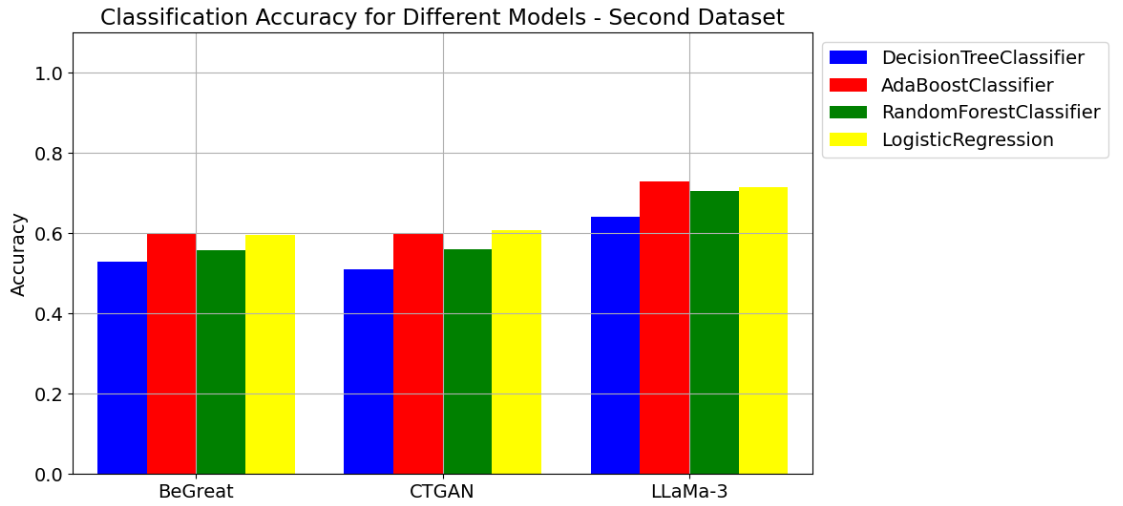
\includegraphics[width=1\textwidth]{images/dataset2_ml.png}
        \caption{Comparison of classification accuracy across machine learning models for the second dataset using Decision Tree Classifier, AdaBoost Classifier, Random Forest Classifier, and Logistic Regression.}
        \label{fig:dataset2_ml}
\end{figure}

Figure \ref{fig:dataset2_ml} shows the performance results of the different machine learning models. It can be observed that CTGAN and the BeGreat model have similar accuracy results. However, the LLaMa-3 model outperforms both the BeGreat and CTGAN models across all machine learning models.





\subsection{Privacy Metrics Comparison}

\begin{figure}[H]
    \centering
        \centering
        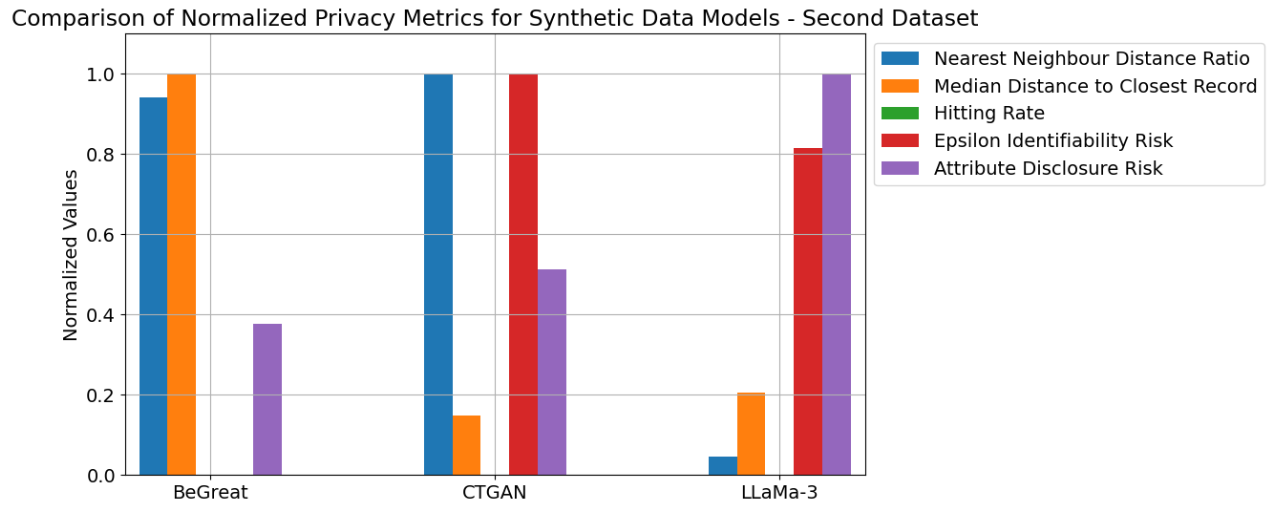
\includegraphics[width=1\textwidth]{images/dataset2_privacy.png}
        \caption{Comparison of normalised privacy metrics for synthetic data models in the second dataset.}
        \label{fig:dataset2_privacy}
\end{figure}


\begin{enumerate}
    \item[(a)] Nearest Neighbour Distance Ratio \\
    The CTGAN model exhibits the highest value among the other models, this suggests a closer generated data to the real data which tends to lower the privacy. On the other hand, the LLaMa-3 model shows a much lower value for this metric suggesting better privacy preservation in terms of distance from real data.

    \item[(b)] Median Distance to Closest Record \\
    CTGAN shows the lowest median distance to the closest record, indicating that the synthetic data is very close to the real data, which might raise privacy concerns. However, both BeGreat and LLaMa-3 have higher values suggesting perfect privacy.

    
    \item[(c)] Hitting Rate \\
    However, all hitting rates are close to the value 0 which indicates that all models contribute to better privacy.


    \item[(d)] Epsilon Identifiability Risk \\
    BeGreat shows the lowest epsilon identifiability risk (0.0002), followed by LLaMa-3 (0.1729). CTGAN has the highest risk (0.2122). CTGAN and LLaMa-3 have around the same risk value, which suggests lower privacy. On the other hand, BeGreat has a value much closer to 0, indicating that it performs better at generating data with a low risk of exposing real information. 

    \item[(e)] Attribute Disclosure Risk \\
    BeGreat shows the lowest attribute disclosure risk, followed closely by CTGAN. LLaMa-3 has the highest risk, indicating lower privacy. However, all models have a relatively high value of the attribute disclosure risk, which suggests they are as vulnerable as the others. %% better reformulation
    
\end{enumerate}



\vspace{1cm}

\noindent \textsc{ \textbf{Summary}}

Overall, the privacy metrics comparison reveals that LLMs tend more to generate data in respect of the data privacy. While CTGAN tends to generate data that is closer to the real data, which raise some privacy concerns.

\vspace{1cm}

\noindent \textsc{ \textbf{Conclusion for the second dataset}}

The utilization of the second dataset has shown that LLMs are more effective in generating data with respect to the real data's distribution, its correlation between variables and its complex structure as indicated by the different metrics and machine learning results. However, LLMs were also able to generate data with better privacy. The GAN-based models, on the other hand, was able to capture the real data's distribution and generate private data but was less performant than LLMs. 




\vspace{10cm}



% Anaylse the impact of different hyperparameters on data quality and realism.

% Discuss the ethical and societal implications of synthetic data generated using LLMs.